\documentclass[conference, a4paper]{IEEEtran}
\IEEEoverridecommandlockouts
\usepackage[left=1.57cm,right=1.57cm,top=0.95cm,bottom=2.54cm]{geometry}

\usepackage[hidelinks]{hyperref}  % PDF Hyperlinks

\usepackage{enumitem}             % Lists
\usepackage{hanging}              % indent

\usepackage{lipsum}               % Lorem Ipsum


\usepackage{siunitx}              % SI Units
\usepackage{booktabs}             % Tables
\usepackage{multirow}
\usepackage{caption}              % Captions


\usepackage{graphicx}             % Images or Graphics
\usepackage{pgfplots}             % Graphs and Plots

% === Change subsection from A B C to 1.1 1.2 1.3 ===
\usepackage{alphalph}
\renewcommand\thesubsectiondis{\AlphAlph{\value{subsection}}.}
\renewcommand\thesubsection{\mbox{\thesection-\AlphAlph{\value{subsection}}}}
% ====================================================



% correct bad hyphenation here
\hyphenation{}



\begin{document}
\title{Smart PowerTrack: Energy Monitoring and Control Socket Relay\thanks{The open-source public repository of this project can be found at \url{https://github.com/vaTomas/PowerTrack/}.}}



% === Authors === %

\makeatletter
\newcommand{\linebreakand}{%
  \end{@IEEEauthorhalign}
  \hfill\mbox{}\par
  \mbox{}\hfill\begin{@IEEEauthorhalign}
}
\makeatother

\author{\IEEEauthorblockN{Vincent Alfred B. Tomas}
\IEEEauthorblockA{\textit{College of Engineering and Architecture} \\
\textit{Mapúa Malayan Colleges Mindanao}\\
Davao City, Philippines \\
vatomas@mcm.edu.ph}
\and
\IEEEauthorblockN{Wrenn Harvyl F. Tajantajan}
\IEEEauthorblockA{\textit{College of Engineering and Architecture} \\
\textit{Mapúa Malayan Colleges Mindanao}\\
Davao City, Philippines \\
whtajantajan@mcm.edu.ph}
\linebreakand
\IEEEauthorblockN{Dale Anthony A. Hemplo}
\IEEEauthorblockA{\textit{College of Engineering and Architecture} \\
\textit{Mapúa Malayan Colleges Mindanao}\\
Davao City, Philippines \\
dahemplo@mcm.edu.ph}
\and
\IEEEauthorblockN{Woodzer L. Plaza}
\IEEEauthorblockA{\textit{College of Engineering and Architecture} \\
\textit{Mapúa Malayan Colleges Mindanao}\\
Davao City, Philippines \\
wplaza@mcm.edu.ph}
}


% The paper headers
\markboth{Microprocessor and Microcontroller Systems and Design~2024}%
{Tomas \MakeLowercase{\textit{et al.}}: Smart Powertrack: Energy Monitoring and Control Socket Relay}


% === Build Title Area  === %
\maketitle


\begin{abstract}
  Electrical power consumption has been a fluent subject of interest since the beginning of the invention of
  induction motors powered by AC currents. This age of time has used its capacity in an extensive level and an
  introduction to a power monitoring system can be introduced. As the flow of electrical power rises,
  consumers tend to unexpectedly use unnecessary electricity that can be reduced when monitored.
  A Smart Power Tracking Socket that is equipped with an Arduino based technology is introduced that aims to
  safely inform users about data concerning their electric power usage in a specified basis.
  The instrument is capable of measuring real-time voltage and current reading in order to calculate power consumption.
  Making the device suitable for users to navigate their personalized information of their consumption as a
  manageable from of responsibility. Second, it is integrated with a relay module that enables to control the
  device upon acted with its corresponding functionality. Whereas, users gain the capability of being in control
  of the device for optimal capacity. It manages to create an appropriate interface for the user to keenly manage
  its device monitoring and controls.
\end{abstract}


% Note that keywords are not normally used for peerreview papers.
\begin{IEEEkeywords}
  Electricity, power, tracking, monitor, control.
\end{IEEEkeywords}







\section{Introduction}
Power and energy are key resources in every household in this day and age. Its importance is at the highest it has ever been and depending on what source the residents are using, it could lead to detrimental effects on the environment. Countless of places primarily use natural resources such as fossil fuels which are limited, costly, and could damage the environment when overused, thus monitoring power and energy consumption is a must \cite{asanza_importance_2023}.
Internationally, numerous countries with high GDP per capita provides their citizens with stronger average purchasing power leading to higher electricity consumptions. Statistics Research Departments states that China consumes the most electricity in the entire world with a per year record of more than 8000 terawatt-hours. Followed by the United States with roughly half with 4000 terawatt-hours and India with 1400 terawatt-hours \cite{statista_research_department_electricity_2024}.
In the Philippines, power monitoring data already existed since 2000 and basing on a national scale that coincides with a data of per capita energy consumption there is a significant increase total energy consumption \cite{enerdata_philippines_2022}. By monitoring our power consumption in our homes, people will be more informed and responsible for their consumption possibly reducing total consumption and translating in to long-term saving.
Seeking an instrument that specializes its function through smart energy control, tracking and monitoring eases the efficiency of daily power consumption. Mainly, it negates the conventional monitoring assumptions and basically deal with real-time measurements of voltage and current to calculate power consumptions. Also, integrates a relay module with IoT technology and Arduino programming that supplies an interface for a user-friendly monitoring and control device.
The project’s primary goal is to build a smart power tracking device that can be use by regular residential consumers of electricity to monitor current flow and help mitigate their energy usage and cost. Enhancing their capability to be control over devices that holds electrical application.

\section{Related Literature}
Through the use of Arduino IDE, the proponents proposed a project about a Smart Power Tracking Socket aiming to monitor and record the power consumption of each appliances through the platform of Arduino IDE while showcasing proficiency and skills with the topic.
The importance of energy monitoring grows day by day that some government across Europe and United States proposed installing smart meters in the future providing immediate feedback on electricity use hoping for an increase in informed citizens and promote changes with regards to their mindset in consuming electricity. The UK government has already committed this by 2019 and concluded that monitoring domestic electricity consumption does seem necessary in reducing consumption levels \cite{webb_antecedents_2014}.
Nowadays, there are countless power monitoring systems in the market. However the affordability and long-term viability of each product is up for debate. Some existing products provide excellent results but costs roughly hundreds if not thousands of us dollars, some provide decent results for a decent price but easily malfunctions, and lastly some couldn’t even produce accurate and consistent results.
From the Fuji Electric, they offer the F-MPC04, a series of devices that offer power distribution and information as well as it serves as an energy monitoring unit. 
It uses four digital inputs, easy to mount switchboards, and supports multiple power distribution lines. It also provides additional features such as identifying the deterioration of insulations and prevent leakage of current. The F-MPC04 series is definitely a great monitoring solution however the main issue for this unit is the pricing. Online stores such as eBay offers a used condition for as low as \$400.00 USD and up to \$1,240.00 USD for a mint condition unit \cite{fuji_electric_fa_components__systems_co_ltd_f-mpc04_nodate}.
Another device found in the market is the Micro Power Monitor Gm86, from Benetech. A device that directly plugs to the outlet to operate and has an LCD display that allows the consumer to monitor the equipment as well as to display the current, voltage, frequency, and active power. For a ₱1000.00 PHP device, it can also records electricity consumption and the total time of use. The main issue for this device is its physical appearance and temperature limit. Appearance-wise it is bulky, when being utilized in a standard socket, the device covers up the outlet rendering it to be useless. It also is limited with the working temperature limit of 0°C to 45°C anything higher or lower may cause the equipment to permanently malfunction or even break \cite{shenzhen_wintact_electronics_co_ltd_micro_nodate}.

\section{Methodology}
This section states and specify the methodology implied to address the designed objective and questions that will potentially provide concrete answers. The proponents utilize a developmental design method in approaching the established questions. Such methods are used to carefully determine programming elements which subscribes to the code commands and language being evaluated in the project. Also, to provide and distinctive comparison of various studies included and marginalizing trial and errors.

\subsection{Design Framework}
The project presents a function block diagram that considered an input-process-output relationship as the conceptual framework as shown in \autoref{fig:design_framework}. In the designed step-by-step function, the input is identified as the dependent and independent conceptual values. Anticipated data defies the processing procedures and the conclusive outcome. The process stage describes how the anticipated data is being analyzed that correspond to indicated required functions. The output corresponds to the displayed information coming from the extracted analyzed variables.

\begin{figure}[tbh]
  \centering
  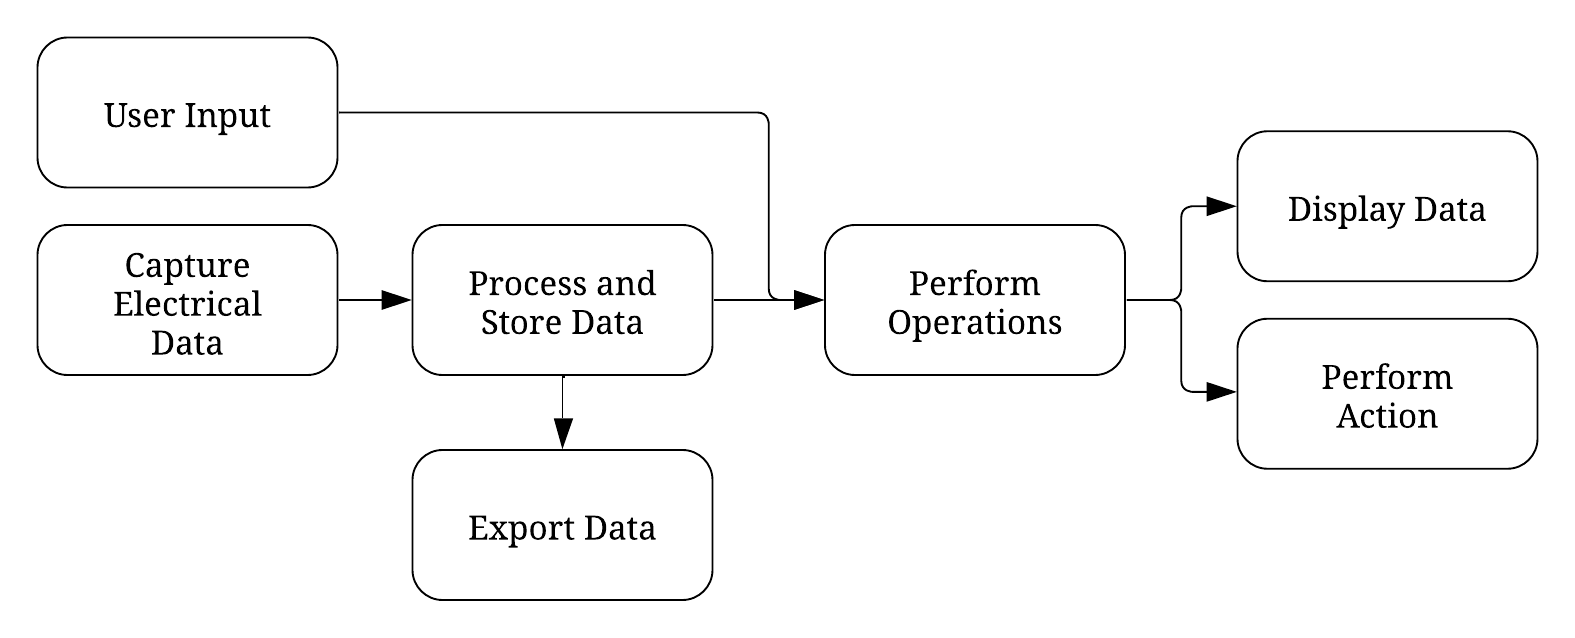
\includegraphics[width=\columnwidth]{img/design_framework.png}
  \caption{Design Framework}
  \label{fig:design_framework}
\end{figure}

In description, Initiating the input variable is necessary to identify the specific data to be considered in the procedures of the programming algorithm. These anticipated variables pertain to the input of data given by two main source of information such as the users input and the captured electrical data. The technology receives this data coming from the amount of electrical energy being produces by a consumer. This data possesses values of the actual voltage and current that is tracked by the socket relay. The values highly depend in the user’s generative consumption of the electrical supply available. Furthermore, it highly reflects the user’s real-time usage and how it may contribute to its energy expenses.

Adding up, the processing aspect of the technology’s function diagram reacts to the data input by the amount that the source provides. Through this, it allows to process and stores the data following the program commands to keep reference for the output display of the algorithm. Given the data necessary for the process, it performs operations that is substantial for the resulting feature that determines the accuracy and precision of the device. This is highly dependent on the input information as it selects appropriate measured variables and solution for the intended displays. Making an efficient characteristic for the operation as it matches capability to the desired output.

The output process produces significant variable that would automatically displays information and performs as its main display. As the device exports its data from its input and processing features, it identifies solutions that would carry conclusions that will perform intended actions through the displayed data information and situational suggestions.

\subsection{Design Philosophy}
This project is guided by a philosophy rooted in safety and open-source principles. Safety is our utmost priority, ensuring that our users have complete peace of mind when using our device. The project firmly stands against any form of unethical behavior and pledge never to store data remotely. The design choices, from software architecture to user interface, are meticulously crafted to create a user-friendly experience. It will offer a straightforward desktop client for ease of use, with data displayed on an LCD and LED indicators. No wireless communication or remote control keeps things simple and secure. Real-time power data, averages, and monthly consumption are at your fingertips, all designed for efficient, eco-conscious living.

\subsection{Design Features}
This project aims to apply the accurate design feature that will sustain a precise prototype that will perform and initiate the desired outputs. This will include concepts that allows users to efficiently control the device. Such features of the Smart Power tracking device will include as showin in \autoref{tbl:design_features}, \autoref{tbl:software_design}, and \autoref{fig:hardware_framework}.

\begin{table}[tbh]

  \centering
  \caption{Design Features}
  \label{tbl:design_features}
  \begin{tabular}{p{0.3\columnwidth}p{0.6\columnwidth}}

      \toprule
      \textbf{Feature} & \textbf{Description}\\
      \midrule
      Power Monitoring & Track power and usage over time \\
      Plug and play & Can run stand alone when powered. No connected desktop required. \\
      Display Statistics & Show power usage and consumption display on the device  \\
      Electrical protection & Each socket is individually fused \\
      Desktop client & Analytics dashboard and configuration \\
      Electrical control & Each socket in individually switched. Customizable routines and quotas. \\
      Prototype & The project is under development and is not in production.\\

      \bottomrule
  \end{tabular}
\end{table}

\begin{table}[tbh]

  \centering
  \caption{Hardware Design}
  \label{tbl:hardware_design}
  \begin{tabular}{ll}

      \toprule
      \textbf{Hardware} & \textbf{Details}\\
      \midrule
      Prototype maximum dimensions & $ \SI{350}{\milli\meter}  \times \SI{100}{\milli\meter} \times \SI{30}{\milli\meter}$ \\
      Maximum AC parameters per scoket & \SI{245}{\volt} and \SI{2}{\ampere} \\
      Number of Power Sockets  & 5 \\
      Socket Type & 3-Prong Universal Power Socket \\

      \bottomrule
  \end{tabular}
\end{table}

\begin{table}[tbh]

  \centering
  \caption{Software Design}
  \label{tbl:software_design}
  \begin{tabular}{ll}

      \toprule
      \textbf{Software} & \textbf{Details}\\
      \midrule
      Software Architecture & Modular Monolithic Architecture  \\
      Programming Language & Arduino / C++, C\# \\
      License & (GNU) General Public License v3.0 \\

      \bottomrule
  \end{tabular}
\end{table}

\begin{figure}[tbh]
  \centering
  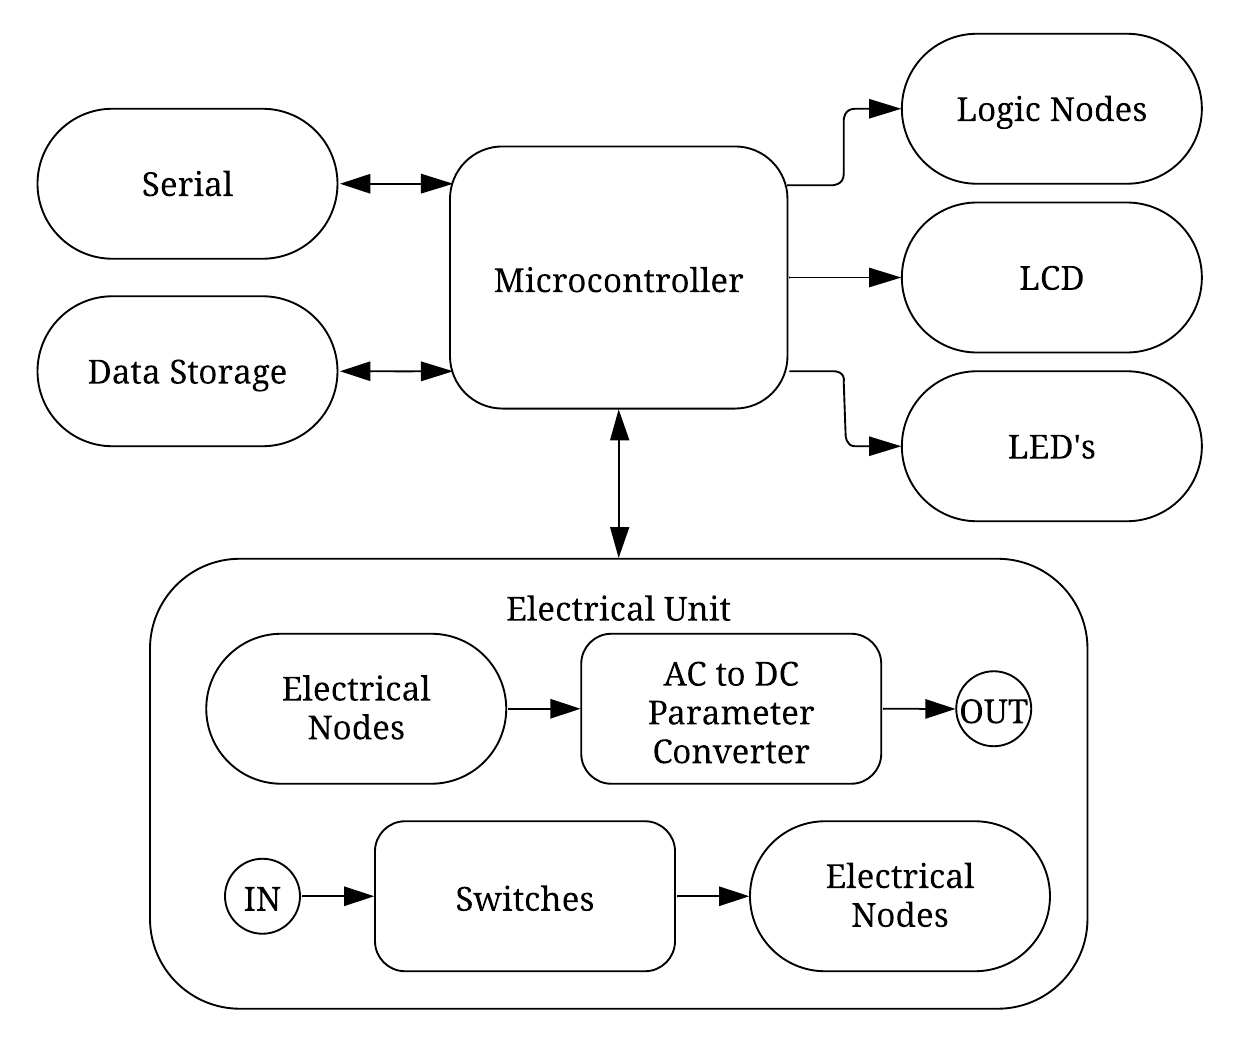
\includegraphics[width=\columnwidth]{img/hardware_framework.png}
  \caption{Hardware Framework}
  \label{fig:hardware_framework}
\end{figure}


\subsection{Design interface}
\subsubsection{User Interface}
User interface will be done through a basic desktop client. Communication between the desktop client and the microcontroller will primarily be done via serial Communication Port (COM), and can be done via SD card.

Input
\begin{itemize}
  \item Tactile toggle button for each power socket.
  \item Mechanical spst switch for the entire system. 
\end{itemize}

Output
\begin{itemize}
  \item LCD display to display historical data.
  \item LED indicators to display current power consumption.
\end{itemize}

Restrictions
\begin{description}
  \item No wireless communication.
  \item No remote control.
\end{description}

\subsubsection{Device Display}
Display Behavior
\begin{itemize}
  \item Turn off display when all sockets hasn’t been disturbed for three (3) minutes to save power.
  \item Turn on display when a socket has been recently disturbed.
  \item Swap between each information to display every five (5) seconds.
\end{itemize}

Information to Display
\begin{itemize}
  \item Real-time Power Draw in Watts (\SI{}{\watt}).
  \item Average 24-Hour Power Draw in Watts (\SI{}{\watt}).
  \item Average Cumulative Power Draw Watts (\SI{}{\watt}).
  \item Average Power Consumption in the past thirty (30) days in (\SI{}{\kilo\watt\hour}).
\end{itemize}

LED Indicators
\begin{itemize}
  \item Each socket must have their own indicator.
  \item Vertical Bar graph beside the socket.
  \item Always On.
\end{itemize}

LED Indicator Modes
\begin{itemize}
  \item Fixed Level - Each bar is preset to a specific wattage.
  \item Adaptive Fixed Level - Each bar is preset to a specific wattage based on usage.
  \item Distribution Share - Each bar is set according to their present share of the current
  total power draw.
\end{itemize}

Restrictions
\begin{itemize}
  \item No Animation.
  \item No Scrolling Text.
  \item No Flashing.
\end{itemize}

\subsection{Main Board}
\label{sec:main_board}

The board has pins for both sides of the PCB. The top has pins for the LCD, reset, I\textsuperscript{2}C buses, SPI bus primarily for the SD card module, extra analog pins,
interrupt, the voltmeter module (ZMPT101B Module), the clock module (DS1302 Module).
The bottom has pins made to attach to the Arduino board acting similarly as an Arduino shield.
The primary part of the board contains five (5) I\textsuperscript{2}C buses that allows the power module to be connected to the main board.
The main bord utilizes a TCA9548APWR IC to multiplex the five (5) power modules to prevent conflicts with the I\textsuperscript{2}C addresses.
Within the board itself users are able to change the address of the I\textsuperscript{2}C multiplexer.
An external real-time clock module will be used to track the datetime due to the limitations of arduino in datetime keeping.
The power input of the entire system will be fused by a \SI{10}{\ampere} ceracmic fuse.

\subsection{Socket Module}
\label{sec:socket_module}
In this project, there are five (5) power modules for each of the five (5) sockets.
There is a solid-state relay (G3MB-202P) and 6 LED's attached to these modules for visualization of the loads for each socket.
There is also one button in each socket to toggle the socket turn on and off, as well as a current sensor IC (ACS712).
The current sensor can detect up to \SI{5}{\ampere} of current, meanwhile the switch can only handle \SI{2}{\ampere} of current.
When the current sensor detects a current greater than or equal to \SI{2}{\ampere} of current, the microcontroller
will send a command to turn off the SSR off. This will act as a dititally controlled fuse for each socket.
For the system fuse, please see \autoref{sec:main_board}.
The current sensor IC cannot be directly connected to the Arduino analog input pins due to the analog-to-digital resolution limitation of the Arduino of only ten (10) bits.
The current sensor IC is then directly connected to a 16-bit an analog to digital converter to increase the resolution to sixteen (16) bits
so the device can sense low value currents.


\begin{figure}[tbh]
  \centering
  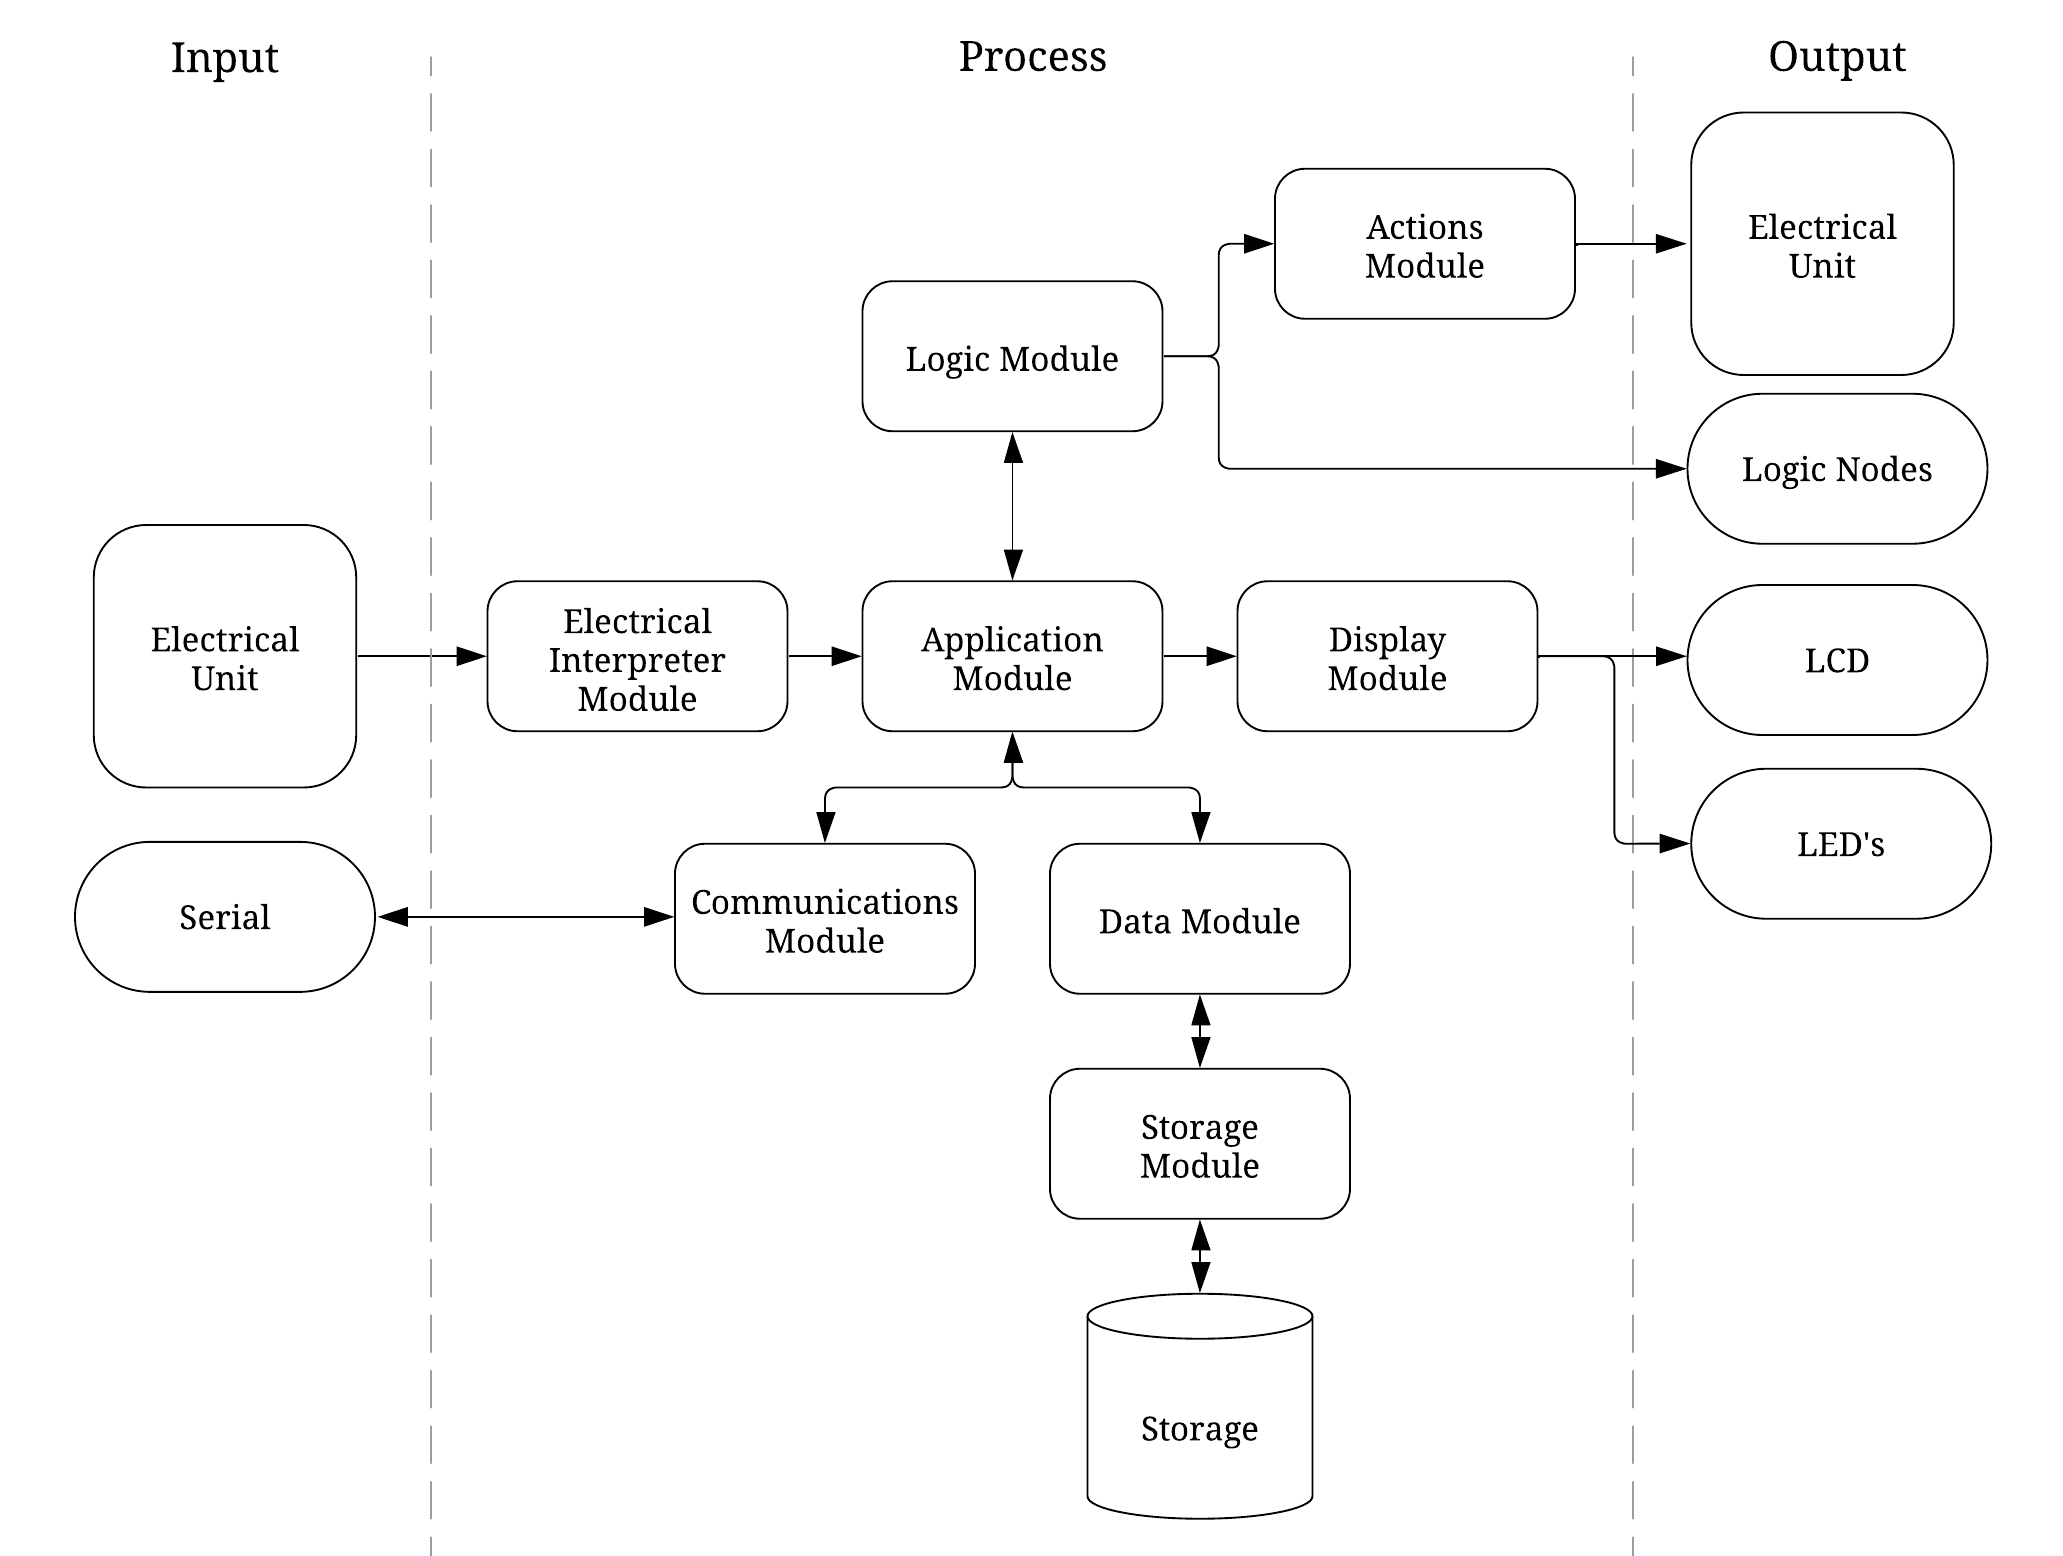
\includegraphics[width=\columnwidth]{img/software_framework.png}
  \caption{Software Framework}
  \label{fig:software_ftamrwork}
\end{figure}

\begin{figure*}[tbh]
  \centering
  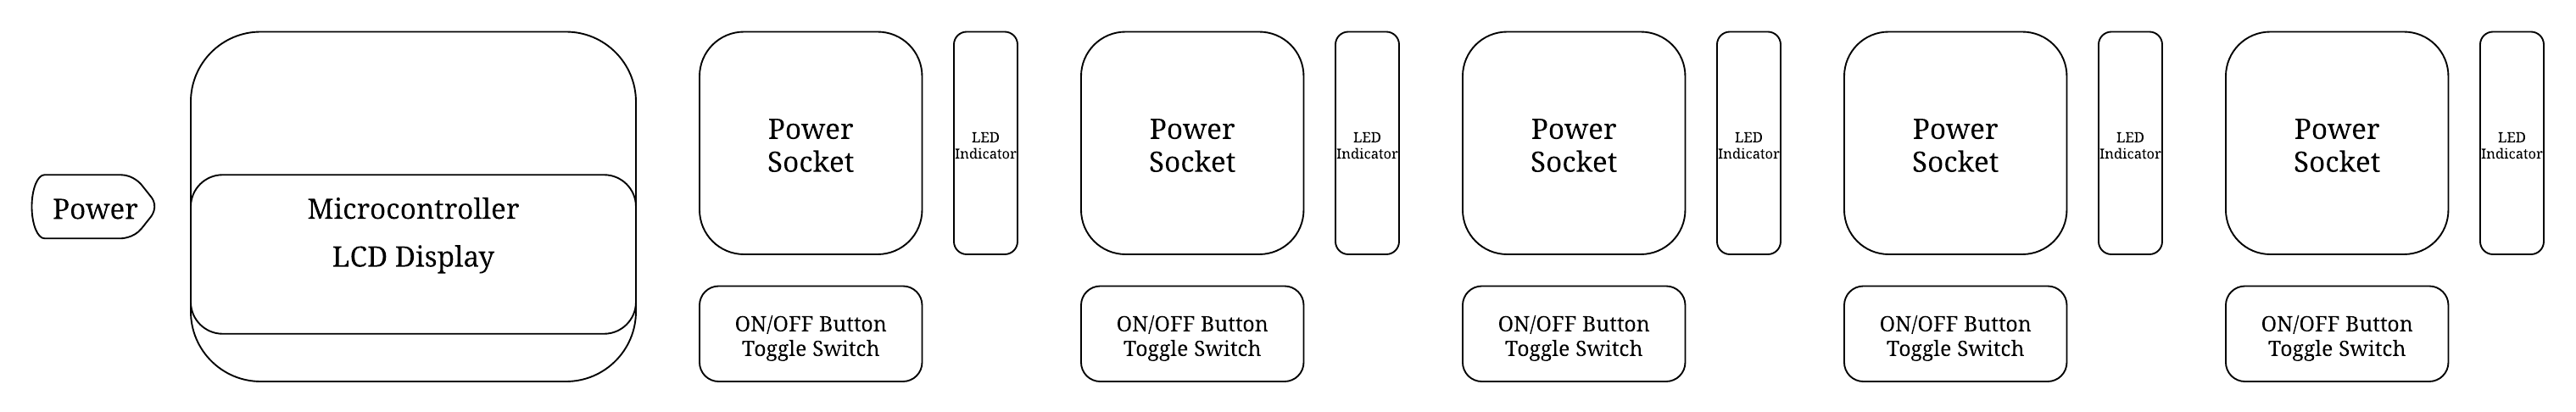
\includegraphics[width=\textwidth]{img/device_layout.png}
  \caption{Device Layout}
  \label{fig:device_layout}
\end{figure*}

\begin{figure*}[tbh]
  \centering
  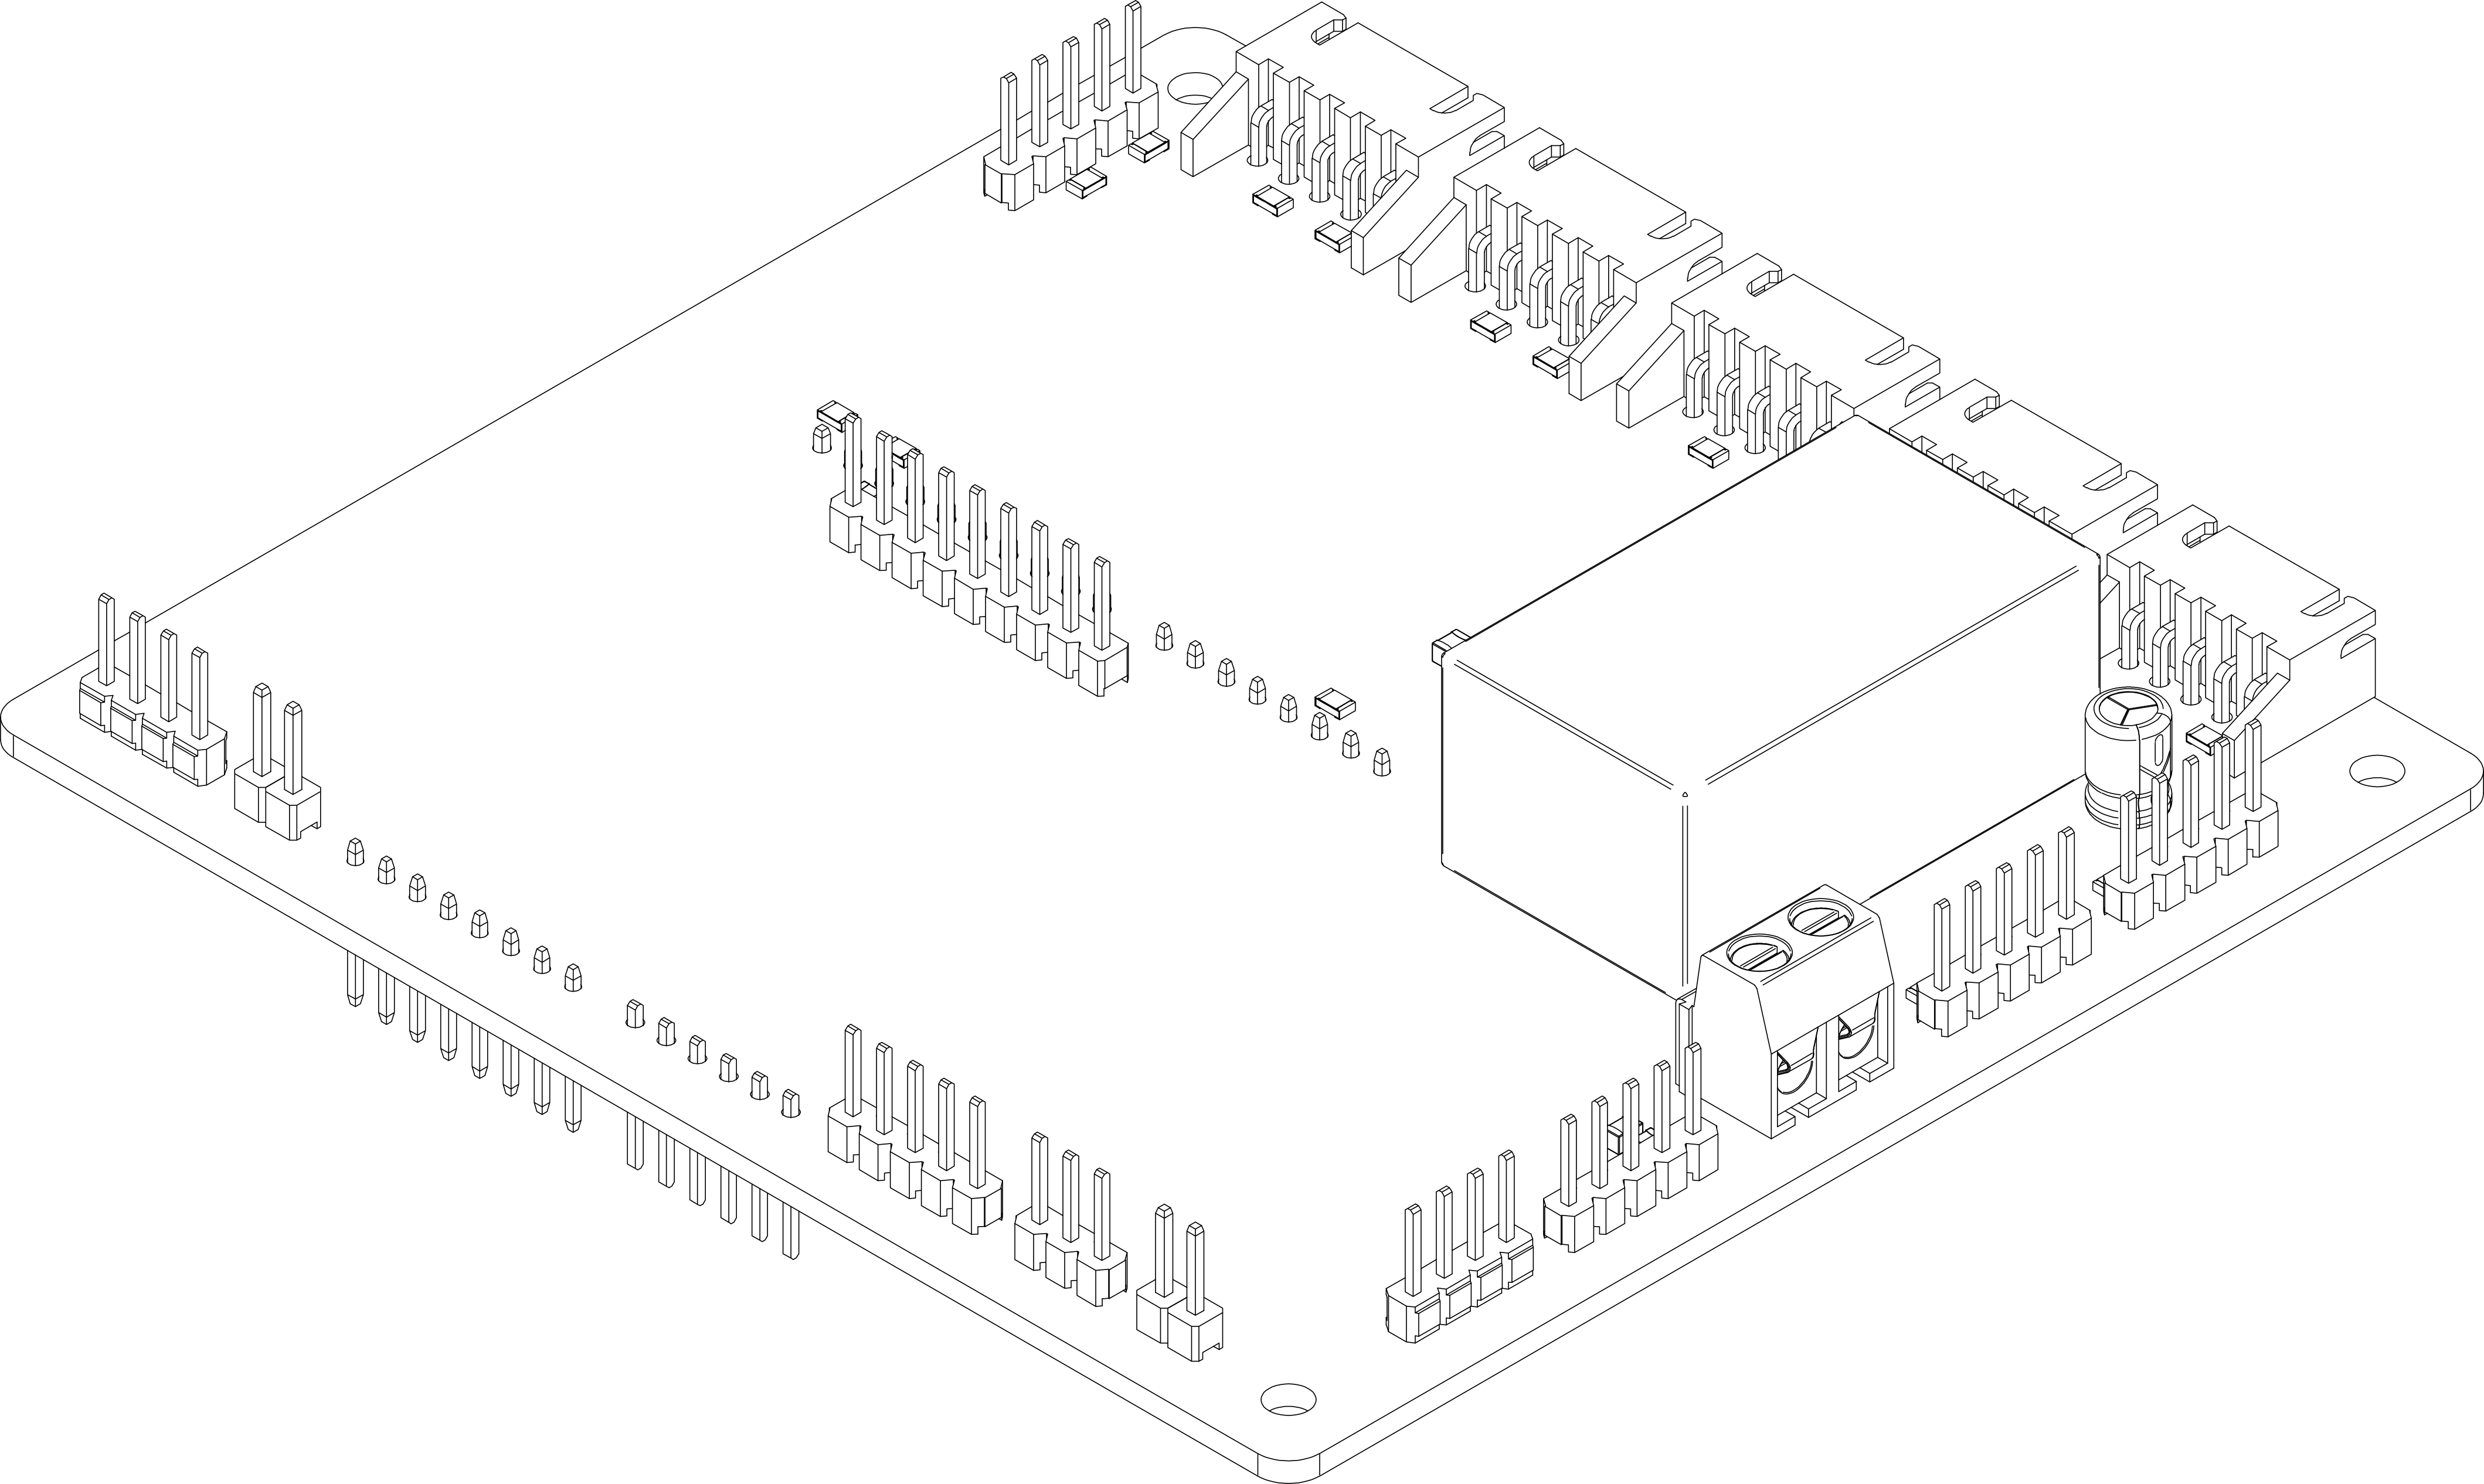
\includegraphics[width=\textwidth]{img/argonarc_wireframe.png}
  \caption{Main Board Isometric View}
  \label{fig:main_board}
\end{figure*}


\begin{figure*}[tbh]
  \centering
  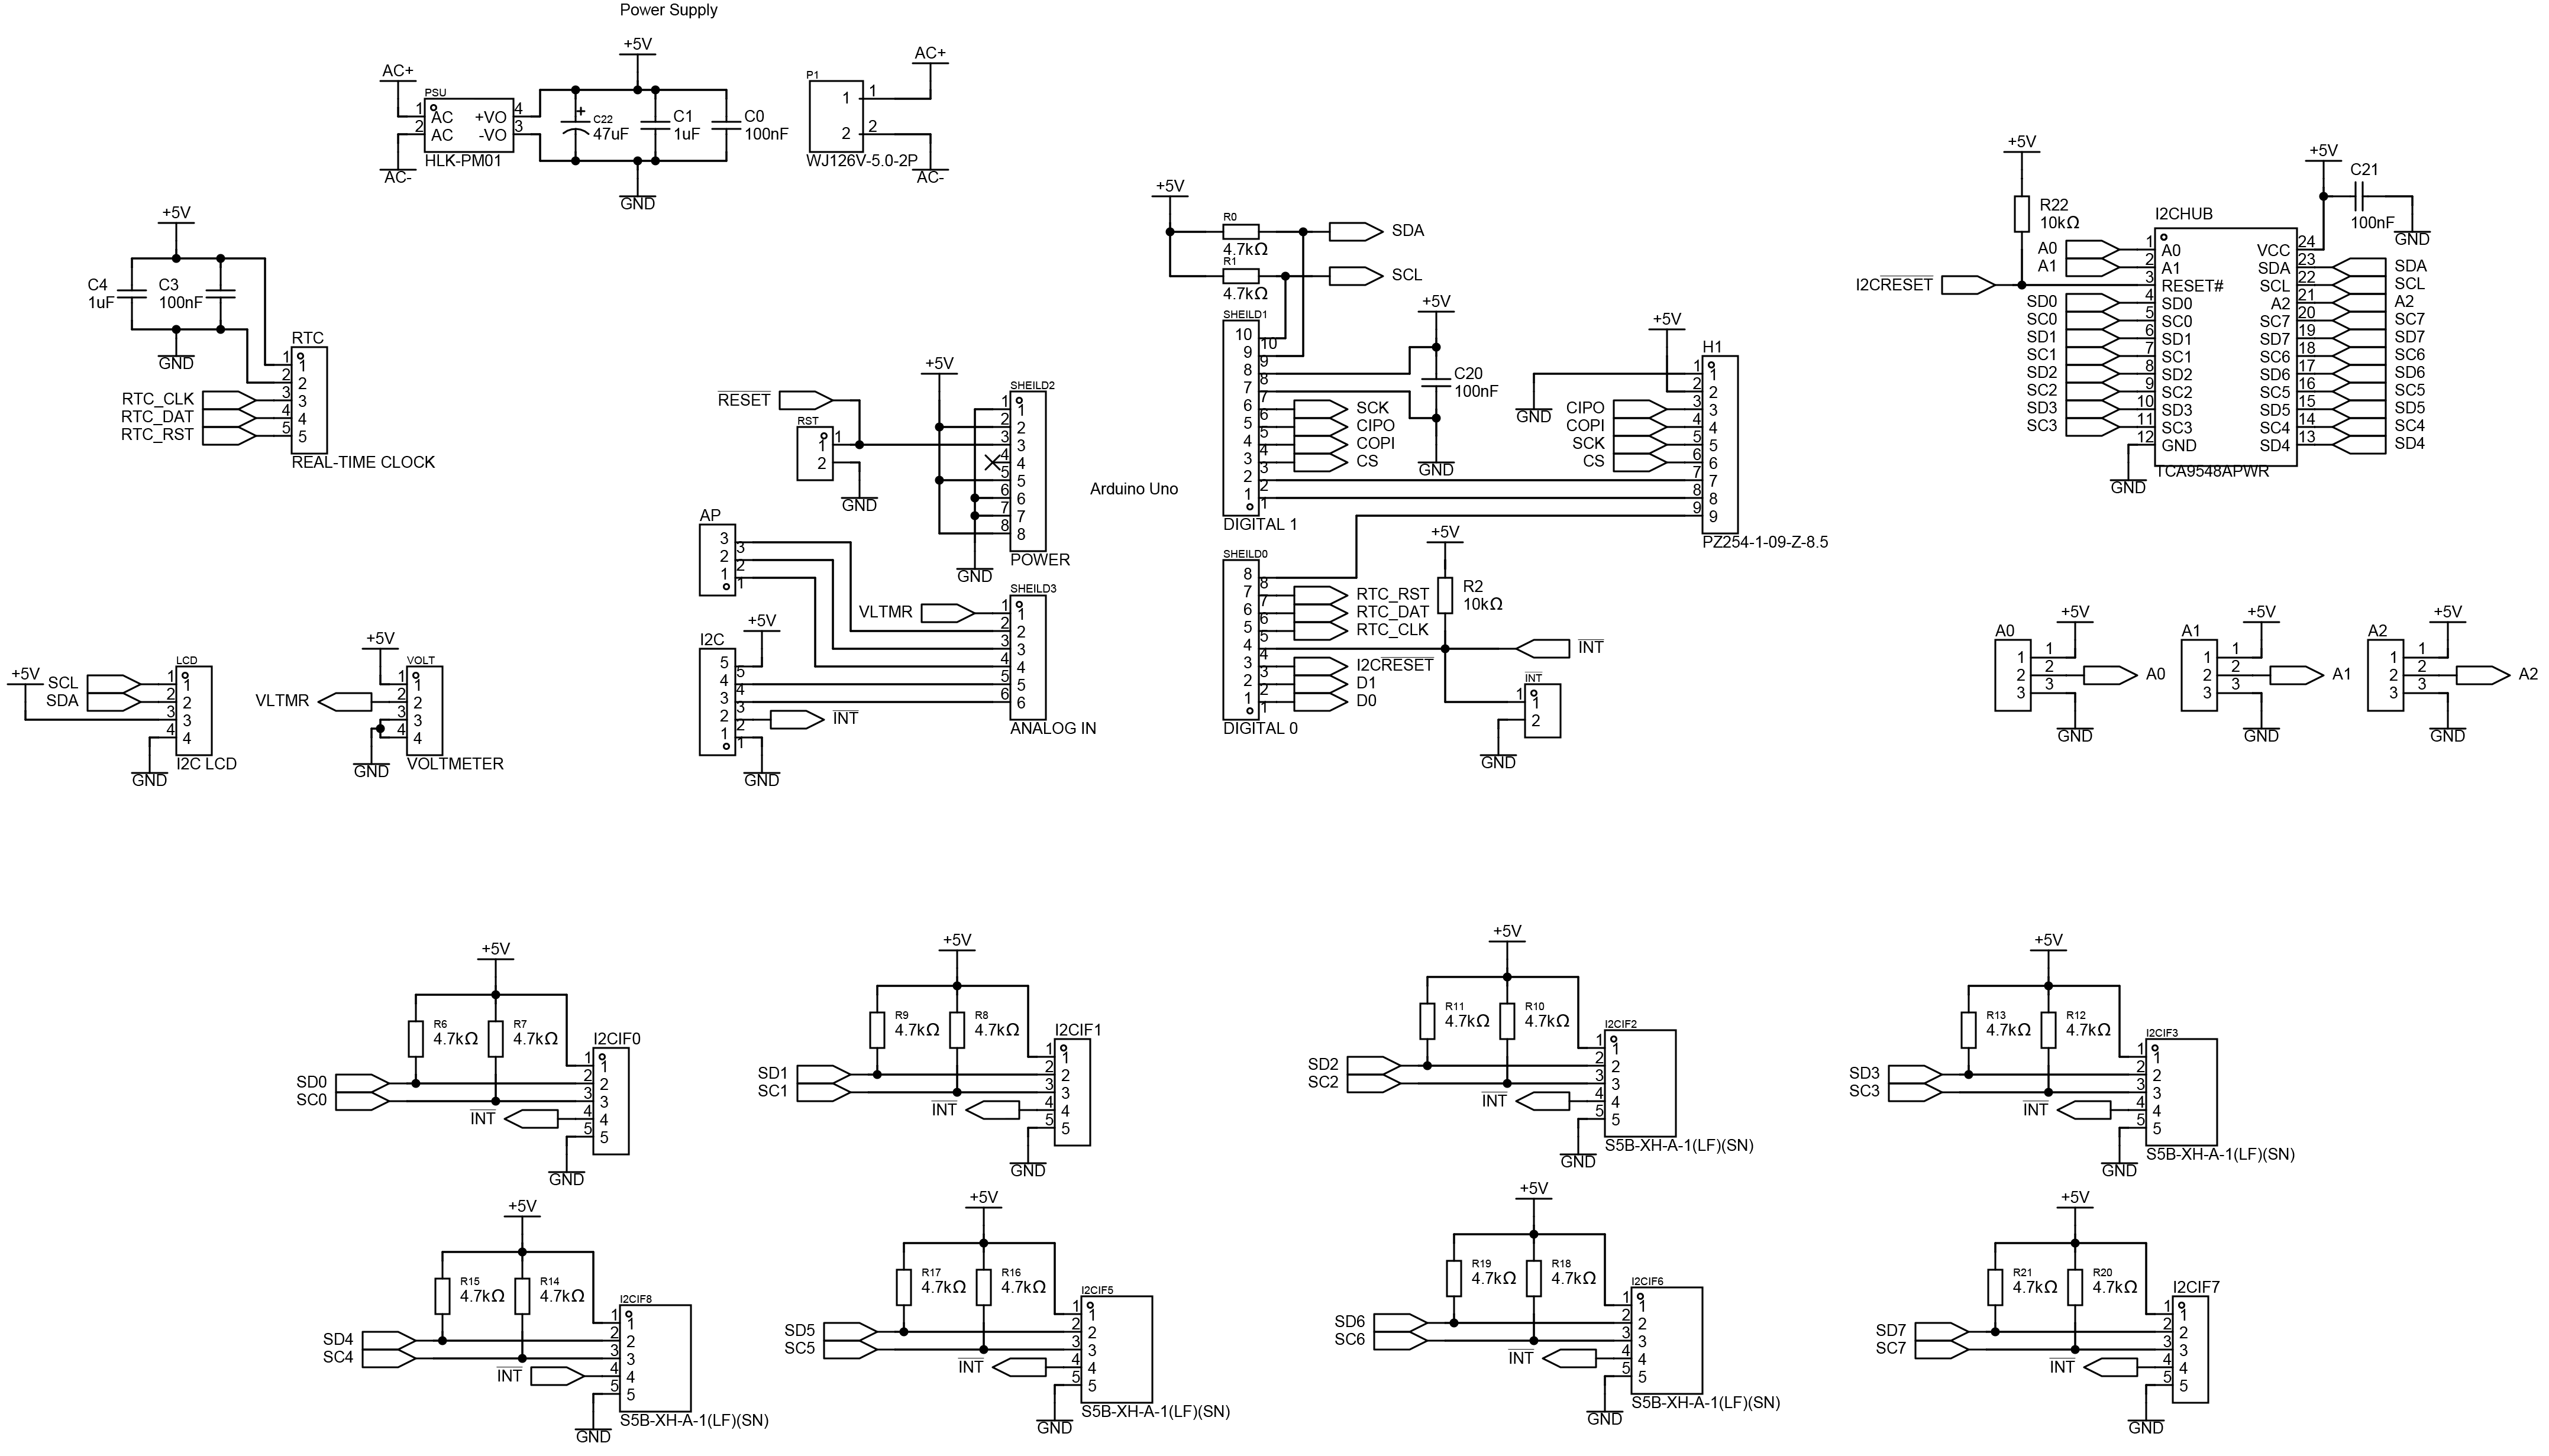
\includegraphics[width=1.4\textwidth,angle=90]{img/board_schematic.png}
  \caption{Main Board Schematic}
  \label{fig:board_schematic}
\end{figure*}

\begin{figure*}[tbh]
  \centering
  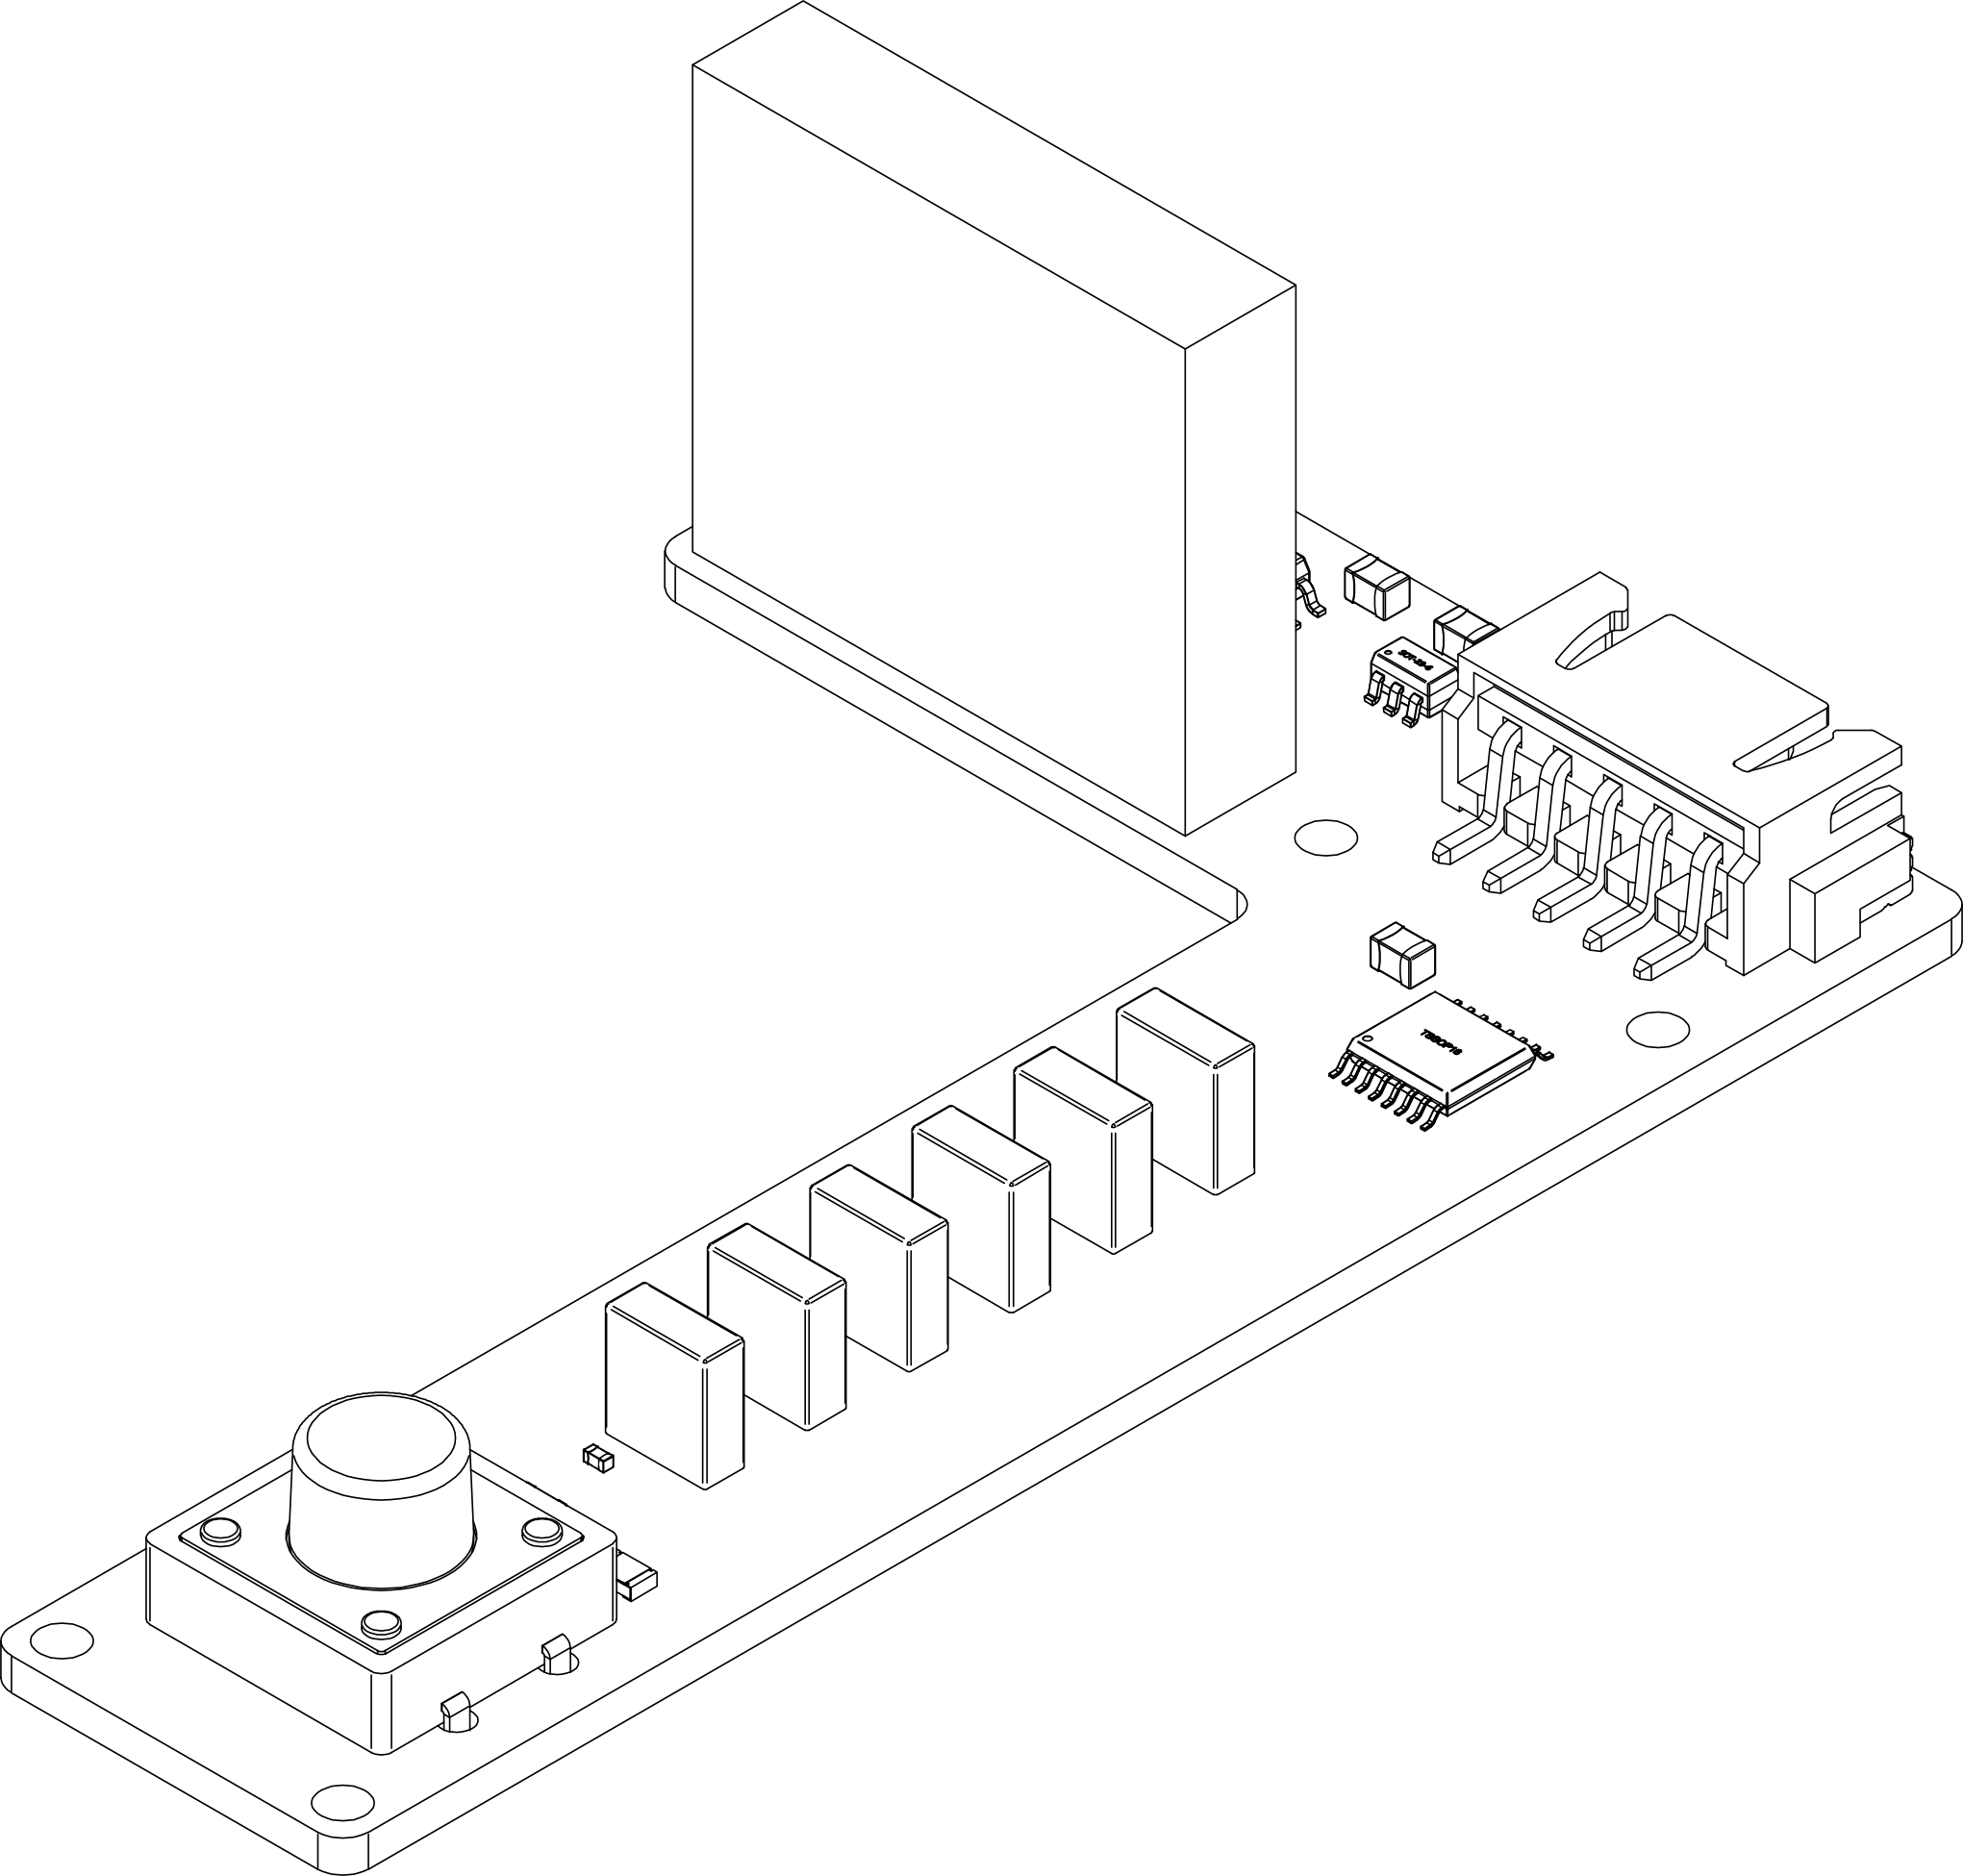
\includegraphics[width=0.48\textwidth]{img/uargonarc_wireframe.png}
  \caption{Power Socket Module Isometric View}
  \label{fig:socket_module}
\end{figure*}

\begin{figure*}[tbh]
  \centering
  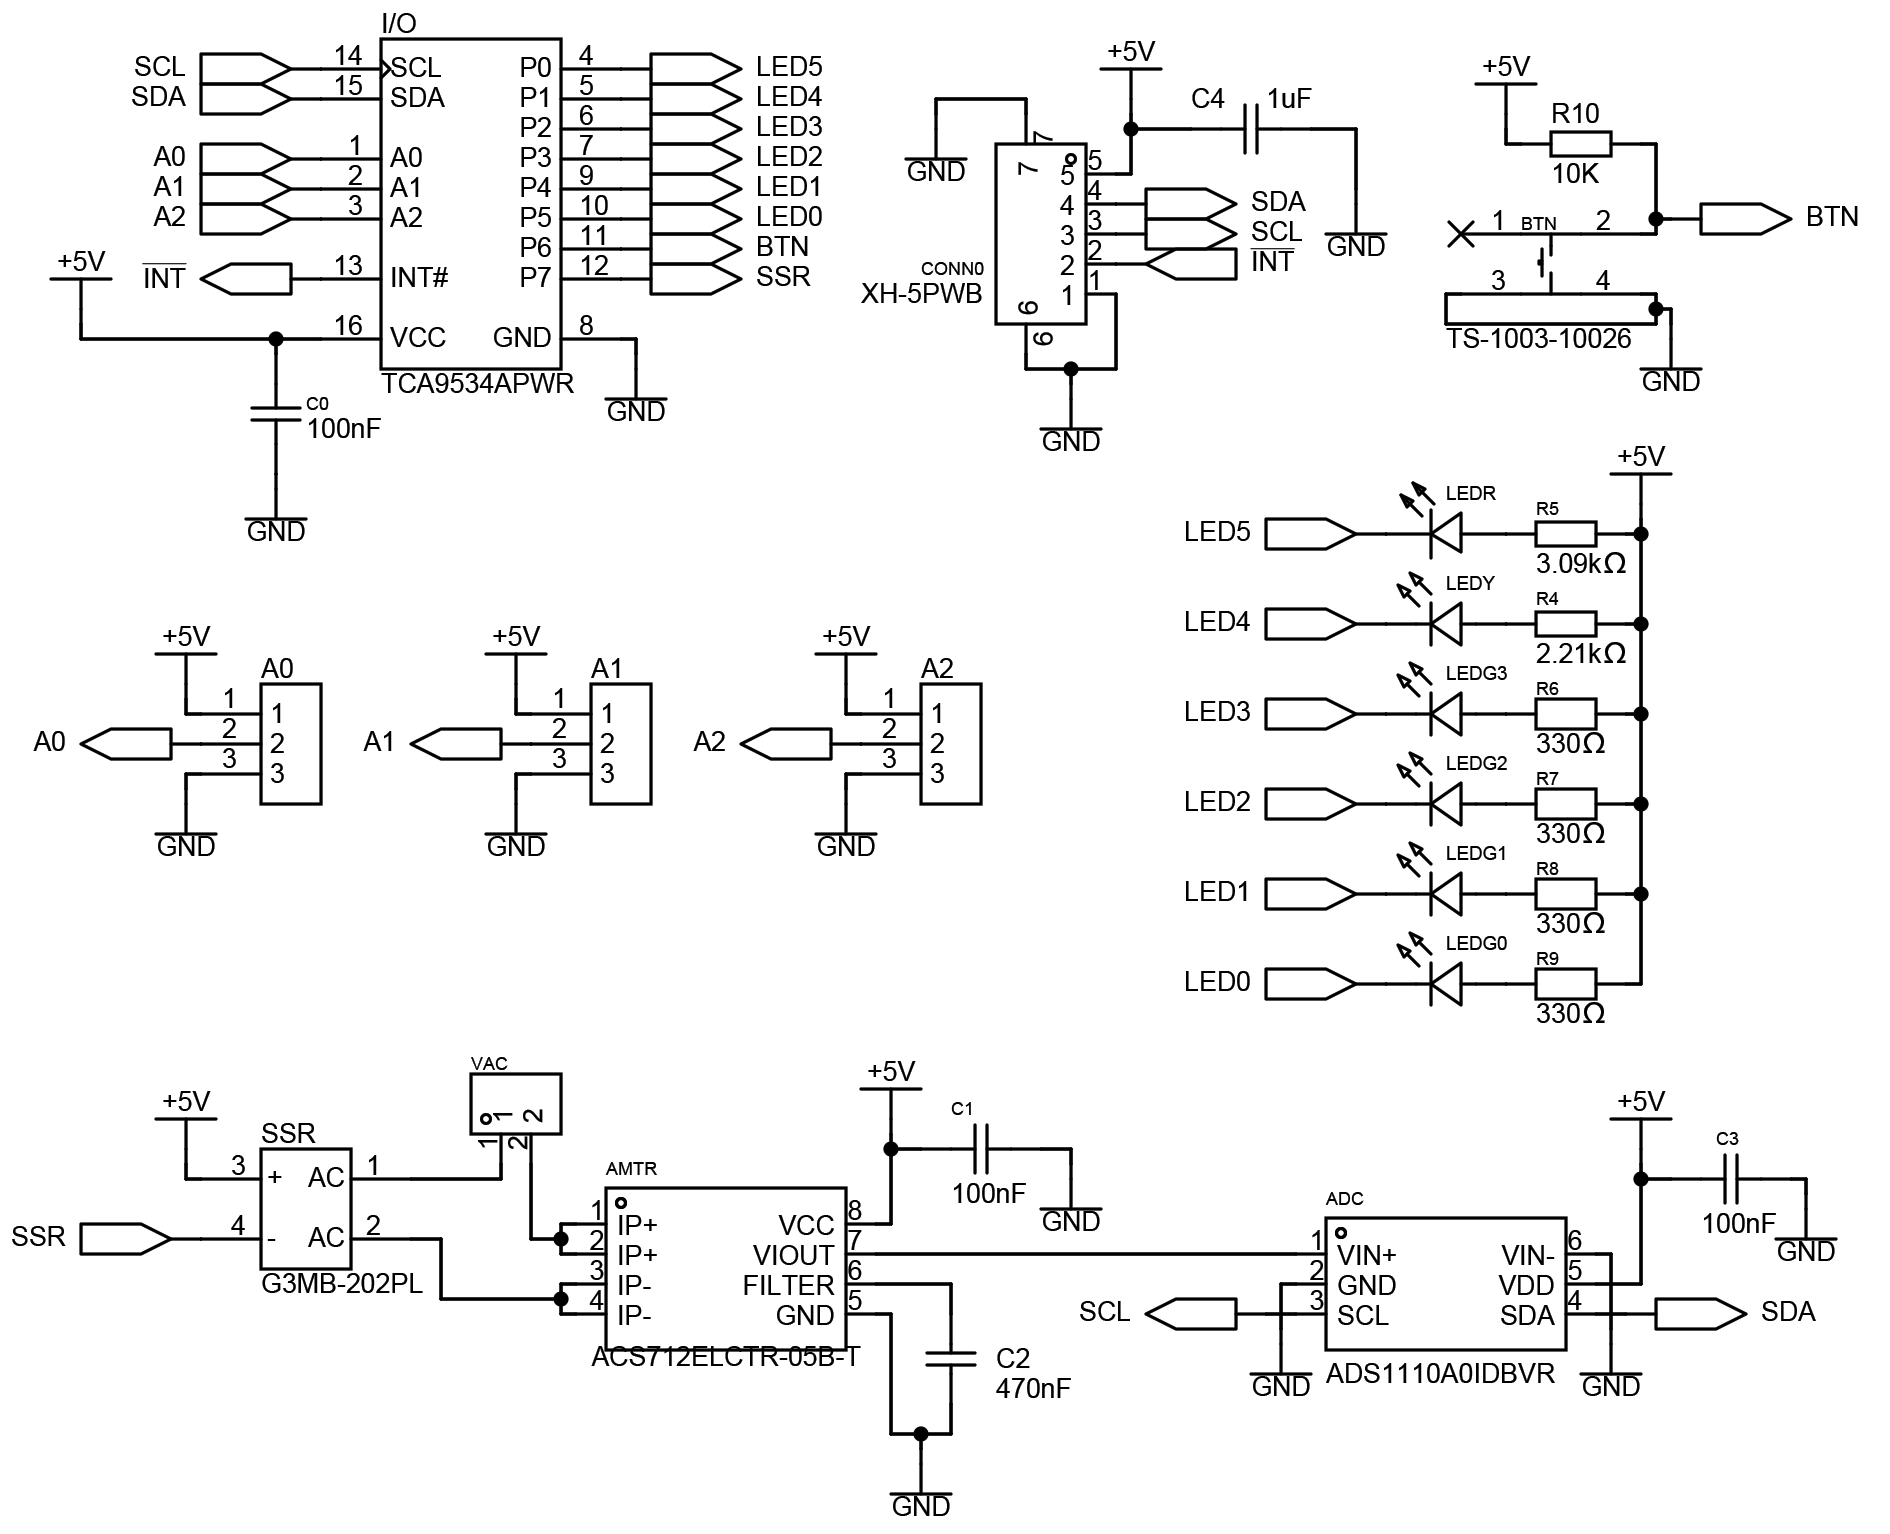
\includegraphics[width=0.8\textwidth,]{img/module_schematic.png}
  \caption{Socket Module Schematic}
  \label{fig:socket_schematic}
\end{figure*}





\section*{Acknowledgment}
The proponents, would like to express their deep and sincere gratitude to all who contributed during the development of this project.
First and foremost, to the group members, colleagues, and families for their support, dedication, and understanding throughout the entirety of the development of this project. The emotional and financial support the proponents received will always be appreciated and served as a source of motivation for the entire development.
Second, to the instructor, Engr. Vince Jebryl G. Montero, who provided the proponents with guidance, support, and feedback throughout the project. His expertise on the topic as well as his support helped the proponents to steer the project into a better path.
Lastly, the proponents are also thankful to the institution, Mapúa Malayan Colleges Mindanao, for providing them with the opportunity to learn all about the course of Microprocessors and Microcontroller Systems. The learning experience has been instrumental towards the completion of the project and will be helpful in their future endeavors.



% Can use something like this to put references on a page
% by themselves when using endfloat and the captionsoff option.
\ifCLASSOPTIONcaptionsoff
  \newpage
\fi


% === Bibliography ===

\bibliographystyle{IEEEtran}
\bibliography{references}

% === End of Bibliography ===


\end{document}


